\section{Equivalência de Recursos}
\label{sec:equivalenciaRecursos}

O conceito de equivalência de recursos refere-se a situações em que recursos distintos podem ser trocados sem perda de função na tarefa sendo executada. Considere o seguinte exemplo:

\begin{quote}
	Lucas estava brincando com seu carrinho, quando uma das rodinhas se quebrou. Entristecido, ele procurou por seu pai, que, ao ver a aflição de seu filho, resolveu ajudá-lo. Recolheu uma garrafa PET que estava por perto, desenroscou sua tampinha e a colocou no lugar deixado pela rodinha estragada.
\end{quote}

O exemplo, apesar de lúdico, apresenta uma situação clara de equivalência entre recursos. Tanto a roda do carrinho como a tampa de garrafa possuem características específicas que as diferem e as individualizam, como material, valor, peso e cor. Além disto, ambas possuem objetivos principais distintos, uma é fechar enquanto a outra é proporcionar mobilidade. Entretanto, as duas têm uma função em comum: são capazes de girar. Sendo esta a função que o carro de brinquedo necessita para o seu funcionamento, os dois objetos tornam-se equivalentes para esta tarefa.

É exatamente esse o sentido ao se afirmar que dois recursos são equivalentes. Um não precisa ser igual ao outro, mas apenas possuir uma característica que, em determinado momento, possibilite a troca de um pelo outro sem perda de funcionalidade. Seria possível, por exemplo, utilizar um \emph{joystick} como um dispositivo apontador e, a qualquer momento, substitui-lo por um \emph{laser pointer} de forma que os serviços necessários continuassem sendo providos. Repare que tais dispositivos, assim como a rodinha e a tampinha, são bastante diferentes em diversas de suas características, mas ainda assim são capazes de fornecer serviços iguais, como mover uma seta pela tela. Caso uma aplicação necessite apenas da capacidade de indentificar localizações em uma tela, um apontador seria suficiente. Neste caso ao se buscar por apontadores no ambiente teríamos como resposta todos os dispositivos equivalentes a essa função (como \emph{mouses}, \emph{joysticks}, \emph{laser pointers} e \emph{trackpads}). Mas no caso de uma aplicação que necessite saber dos movimentos do usuário (como o gesto de \emph{pinch-zoom}, pinça com os dedos) apenas o \emph{trackpad} seria adequado. Para que isto seja possível é necessário conhecer como é estabelecida a relação de equivalência.

\subsection{Relação de Equivalência}

Para que determinado recurso seja equivalente a outro, deve-se garantir que as 3 regras a seguir sejam sempre respeitadas. Para tal, admita que a notação $A \implies B$ denote que um recurso A é equivalente a um recurso B.

\begin{enumerate}
	\item Consistência de serviços

		Entende-se por consistência de serviços a garantia de que o recurso equivalente contenha em sua definição, além dos seus próprios serviços, todos daqueles presentes na classe à qual ele se diz equivalente. Portanto, caso $R1 \implies R2$, os serviços providos por R2 devem existir em R1.
	\item Consistência de interface

		Entende-se por consistência de interfaces a garantia de que dois ou mais serviços existentes em recursos distintos possuam nomes e parâmetros iguais. Portanto, caso $R1 \implies R2$, as interfaces dos serviços providos por R2 que também estão em R1 devem ser idênticas.

		Parte-se do princípio que não existirá interesse em camuflar um serviço malicioso ao expor uma interface compatível com a equivalência.
	\item Referência circular

		Para a ocorrência de equivalência, é necessário a existência de uma classe inicial, à qual outros recursos possam se afirmar equivalentes. Neste caso, é necessario que não haja ciclos nessas referências, de tal forma que seja possível encontrar a classe original.

		Por definição, são necessárias pelo menos duas classes distintas para a possibilidade de ocorrência de uma referência circular.
\end{enumerate}

Desta forma a relação de equivalência é:

\begin{itemize}
	\item Reflexiva: $R1 \implies R1$;

	\begin{itemize}
		\item Prova \\

		Sejam R1 e R2 recursos quaisquer tais que $R1 = R2$. Considere que S(X) represente o conjunto de serviços contidos no recurso X, que S($X \cap Y$) represente o conjunto resultante da intercessão dos serviços existentes em X e Y e que I(S(X)) seja o conjunto de interfaces dos serviços presentes em X. Logo: \\
		
		\begin{enumerate}
			
			\item $S(R1 \cap R2) = S(R2)$; \\
			\item $I(S(R1 \cap R2)) = I(S(R2))$; \\
			\item A quantidade de recursos distintos envolvidos é menor do que 2. Portanto não existe referência circular.
		\end{enumerate}
		\begin{flushright}$\Box$\end{flushright}
	\end{itemize}
	
	\item Não-simétrica: se $R1 \implies R2$ e $R1 \neq R2$, então o inverso não é verdade;

	\begin{itemize}
		\item Prova \\

		Sejam R1 e R2 recursos quaisquer tais que $R1 \neq R2$. \\

		\begin{enumerate}
			\item $S(R2 \cap R1) \neq S(R1)$; \\
		\end{enumerate}

		Pela falha da primeira regra, percebe-se que o recurso R2 não é equivalente a R1.
		\begin{flushright}$\Box$\end{flushright}
	\end{itemize}

	\item Transitiva: se $R1 \implies R2$ e $R2 \implies R3$, então $R1 \implies R3$.

	\begin{itemize}
		\item Prova \\

		Sejam R1, R2 e R3 recursos quaisquer tais que $R1 \implies R2$ e $R2 \implies R3$ e $R1 \neq R2$, $R2 \neq R3$ e $R1 \neq R3$. \\

		\begin{enumerate}
			
			\item $S(R2 \cap R3) = S(R3)$. Mas $S(R1 \cap R2) = S(R2)$. Logo, $S(R1 \cap R3) = S(R3)$; \\
			\item $I(S(R2 \cap R3)) = I(S(R3))$. Mas $I(S(R1 \cap R2)) = I(S(R2))$. Logo $I(S(R1 \cap R3)) = I(S(R3))$; \\
			\item $S(R2 \cap R1) \neq S(R1)$, $S(R3 \cap R2) \neq S(R2)$ e $S(R3 \cap R1) \neq S(R1)$.
		\end{enumerate}
		\begin{flushright}$\Box$\end{flushright}
	\end{itemize}	
\end{itemize}

\subsection{Árvore de Recursos}
\label{subsec:arvoreDeRecursos}

Para que fosse possível validar as relações de equivalências propostas, fez-se necessária a criação de uma estrutura capaz de relacionar os tipos básicos com os seus subtipos. Tal estrutura deve permitir uma boa organização lógica dos tipos relacionados e facilitar a navegabilidade entre eles. Dessa forma, criou-se uma representação em que cada um dos tipos básicos (Seção~\ref{sec:tiposBasicos}) servirá de raiz para uma árvore de recursos, ou seja, existirão diversas árvores, cada qual com outros tipos agrupados por funcionalidades formando um grafo desconexo. Dessa forma, toda definição de \emph{driver} ou declara explicitamente a quais outros \emph{drivers} ele é equivalente ou não declara nenhum e se torna uma nova raiz. Para tornar tal estrutura mais clara, considere a Figura~\ref{fig:arvoreDeRecursos}. Observe a hierarquia formada a partir do tipo básico \emph{Pointer}. Ele é responsável por agrupar todas as classes de recursos capazes de prover serviços relacionados aos apontadores existentes, por exemplo, \emph{click} e \emph{scroll}. O mesmo acontece com os demais tipos básicos.

\begin{figure}[ht]
	\center
	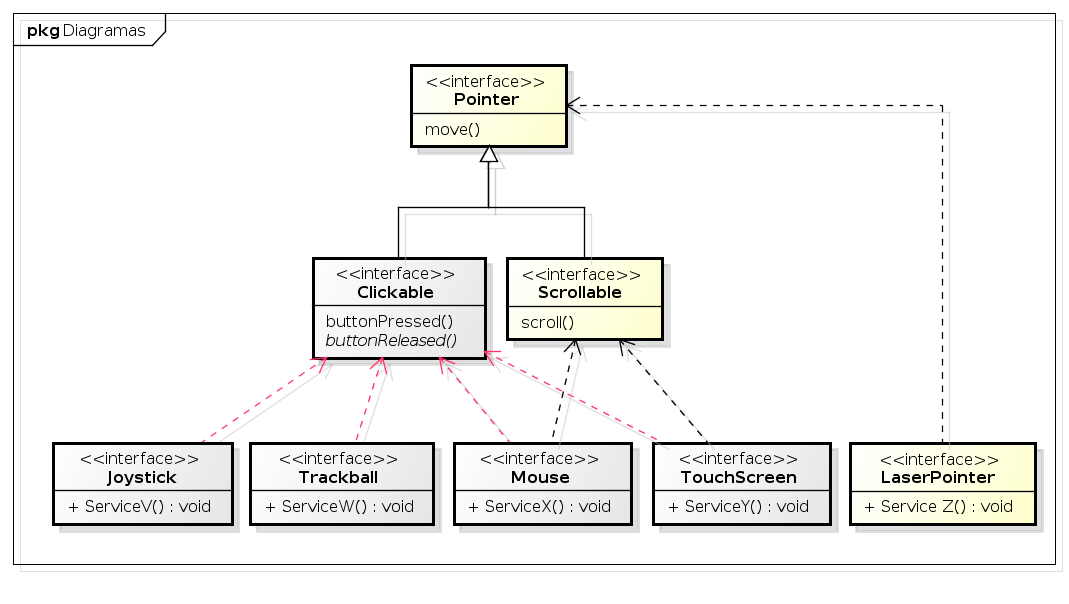
\includegraphics[scale=0.55]{imagens/arvoreDeRecursos}
	\caption{Exemplo de uma das árvores de recursos.}
	\label{fig:arvoreDeRecursos}
\end{figure}

Uma vez que tal estrutura esteja construída, para descobrir todos os recursos equivalentes a quaisquer tipos presentes na árvore, basta tomar a sub-árvore cuja raiz é o elemento ao qual deseja-se obter seus equivalentes. Quanto mais próximo da raíz, mais genérico será o recurso, e à medida que se aproxima das folhas da árvore, mais específico será o recurso. Tomando o exemplo da Figura~\ref{fig:arvoreDeRecursos} considere que seja necessário oferecer todos os recursos equivalentes ao tipo \emph{Clickable}. Ao se colocar tal tipo como raiz de sua sub-árvore, torna-se fácil perceber que os tipos \emph{Joystick}, \emph{Trackball}, \emph{Mouse} e \emph{TouchScreen} são seus equivalentes. A Figura~\ref{fig:arvoreDeRecursos} mostra ainda situações de herança múltipla, em que \emph{Mouse} e \emph{TouchScreen}, além de possuírem os serviços do tipo \emph{Clickable}, possuem também serviços do tipo \emph{Scrollable}. A definição de novos recursos deve respeitar a interface do tipo herdado. Essa condição já é garantida pela utilização de herança de interfaces Java.
